\chapter{Projektafgrænsning}
%afgrænsninger i projektet her.

Et fuldt integreret vandingssystem er, grundet manglende ressourcer og tid, ikke en mulighed på dette semesterprojekt, men der udarbejdes i stedet en skaleret prototype. Det vil sige at der i alt implementeres én Master og én Enhed med tilhørende komponentpakke og sprinkler. 
Foruden størrelsesbegrænsning er der fra skolens side givet forbud mod, uanset tidligere baggrund, at der arbejdes på 230 VAC. Men da der indgår en 230 VAC pumpe i projektet har skolen givet særtilladelse til at der laves et relæ-kredsløb i en lukket kasse, hvori alle ledende dele er helt afskærmet for fysisk kontakt som kan ses på figur \ref{lab:230Vrelay}.

Hurtigt i projektets forløb fik vi tildelt en pumpe fra Grundfos, det viste sig senere at denne ikke kunne bruges til det ønskede formål med at skabe et vandtryk, da denne er en cirkulationspumpe. 

%Løsningen på dette ender med en billig vandpumpe til påmontering på en 230 V %boremaskine. 

\begin{figure}[H]
  \centering
    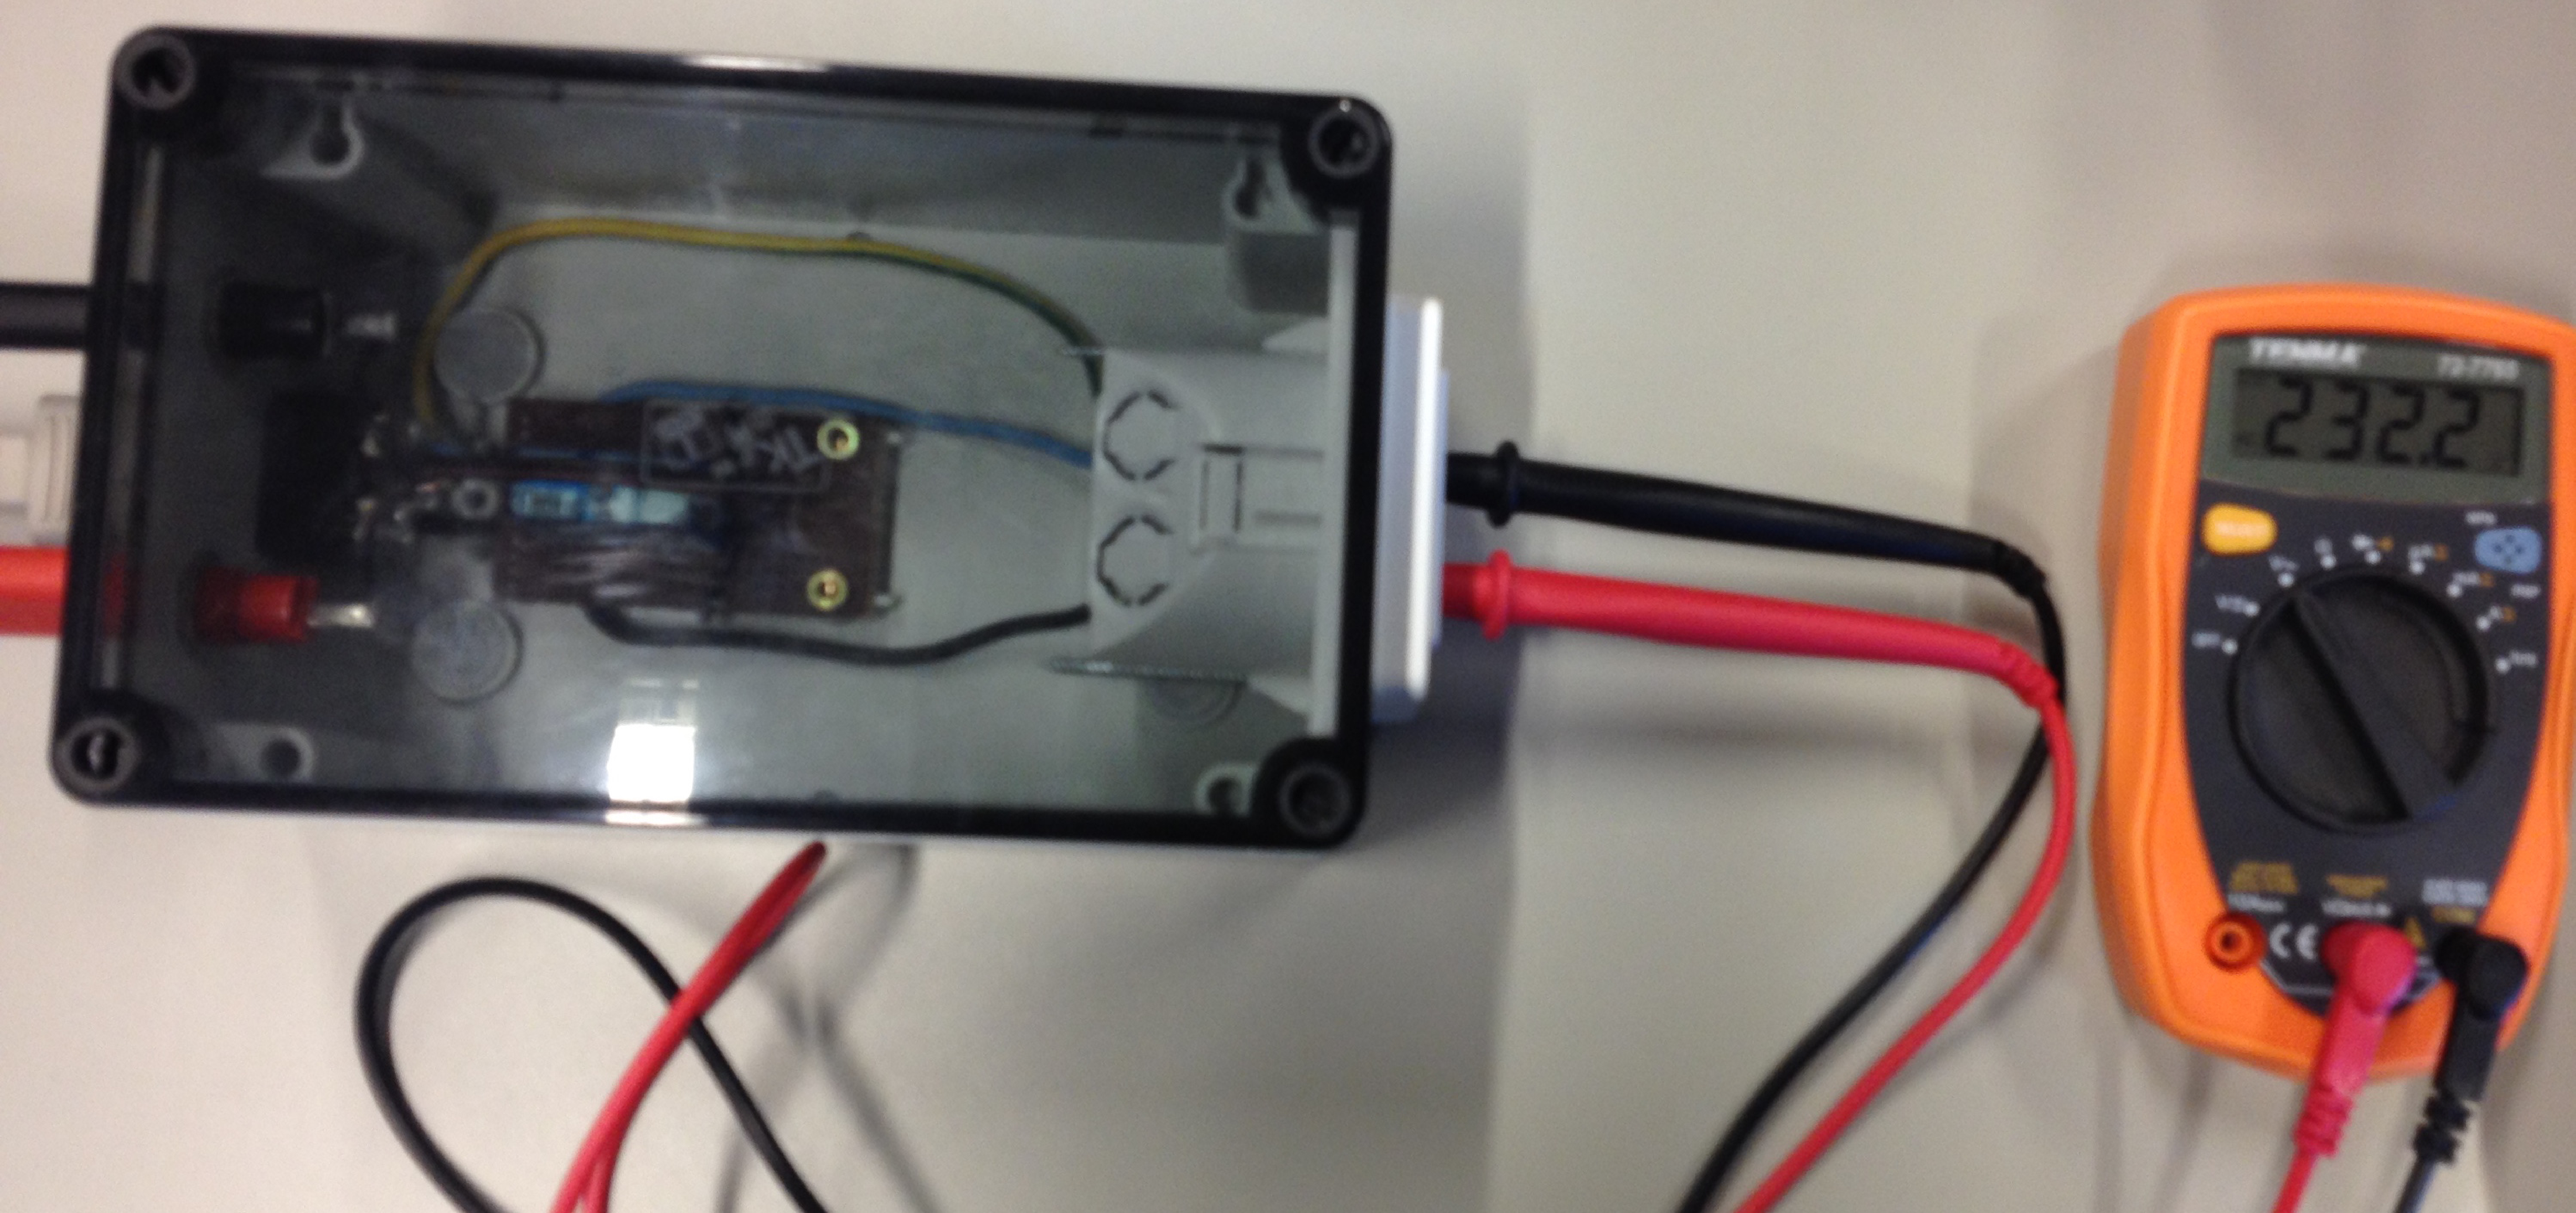
\includegraphics[width=0.75\textwidth]{Billeder/230Vrelay}
    \caption{Relæ i afskærmet kasse. Multimeteret måler 230 V på udgangen.}
    \label{lab:230Vrelay}
\end{figure}

Efter at den serielle kommunikation (SPI) var implementeret færdig og klar til test, viste det sig at overførelsesafstanden på 22 cm, som først var tiltænkt, ikke kunne lade sig gøre, da dataen blev korrupt undervejs. Denne afstand blev da nedsat til 7 cm for at kunne overføre data uden fejl.
 
I softwareimplementeringen er der tiltænkt en  avanceret fejl-håndtering og filstruktur til at gemme opsætning- og logdata på Devkit8000. På grund af at vi mistede en software-mand i gruppen er disse ting udeladt til fordel for at få den grafiske brugerflade og den autonome funktionalitet op at køre. Dette har resulteret i at alle fejlbeskeder på den grafiske brugerflade ikke er implementeret.

Prototypen udvikles med nogle andre tidsintervaller end dem specificeret i kravspecifikationen. Dette skyldes at vi gerne vil kunne se systemet virke i lille skala og i test øjemed.

Tiderne er som følger.

\begin{itemize}
	\item Datalogning fra Enheder på Master hvert 15. sekund
	\item Datalogning og autonom reaktion på Enheder hvert 8. sekund
	\item Afbrydelse af autonomt system ifm. bevægelse: 20 sekunder
\end{itemize}